
\chapter{Introduction}
\setcounter{page}{1}
\pagestyle{plain}

Spoken language is one of the most powerful systems of communication at our disposal. A large part of our waking hours is spent in social interactions mediated through natural language.  The central role of spoken language in our daily lives is largely due to its remarkable ability to convey (sometimes highly elaborate) ideas in a robust and efficient manner. 

Is it possible to exploit this basic fact to develop more user-friendly technologies? Most of our everyday activities are now relying on ``smart'' electronic devices of various kinds, from mobile phones to personal computers and navigation systems. As these technologies gain in autonomy and sophistication, the design of appropriate user interfaces becomes increasingly important. Human-computer interfaces should provide the user with rich and flexible interaction channels, yet remain easy to understand and control.  One natural way to achieve this goal is to endow computers with a capacity to understand, even if in a limited manner, the communication medium that is most intuitive to human beings, namely spoken language.  

The ongoing research on \textit{spoken dialogue systems}\index{spoken dialogue systems} (SDS) is precisely trying to realise this objective. A spoken dialogue system is a computational agent that can converse with humans through everyday spoken language. Such systems are expected to play an ever-increasing role in our interactions with technology. They have a wide spectrum of applications, ranging from voice-enabled mobile applications to in-car navigation assistants, smart home environments, tutoring systems, and (in a not-too-distant future) service robots assisting us in our daily chores.

Figure \ref{fig:basicsds} depicts an example of interaction between a human user and a spoken dialogue system. When the user starts talking, the system extracts the corresponding speech signal through a microphone.  The speech signal is then processed to analyse its content.  Once this analysis is completed, the system must determine how to react.  In this case, the system decides to greet back the user and selects the words to express it (\utt{good morning, sir}). The final step is to synthesise these words through an artificial voice, which closes the loop.\footnote{ Needless to say, the schema hides a great deal of internal complexity.  The next chapter describes in more detail the software architectures used to design practical spoken dialogue systems.}

\begin{figure}[ht]
\center
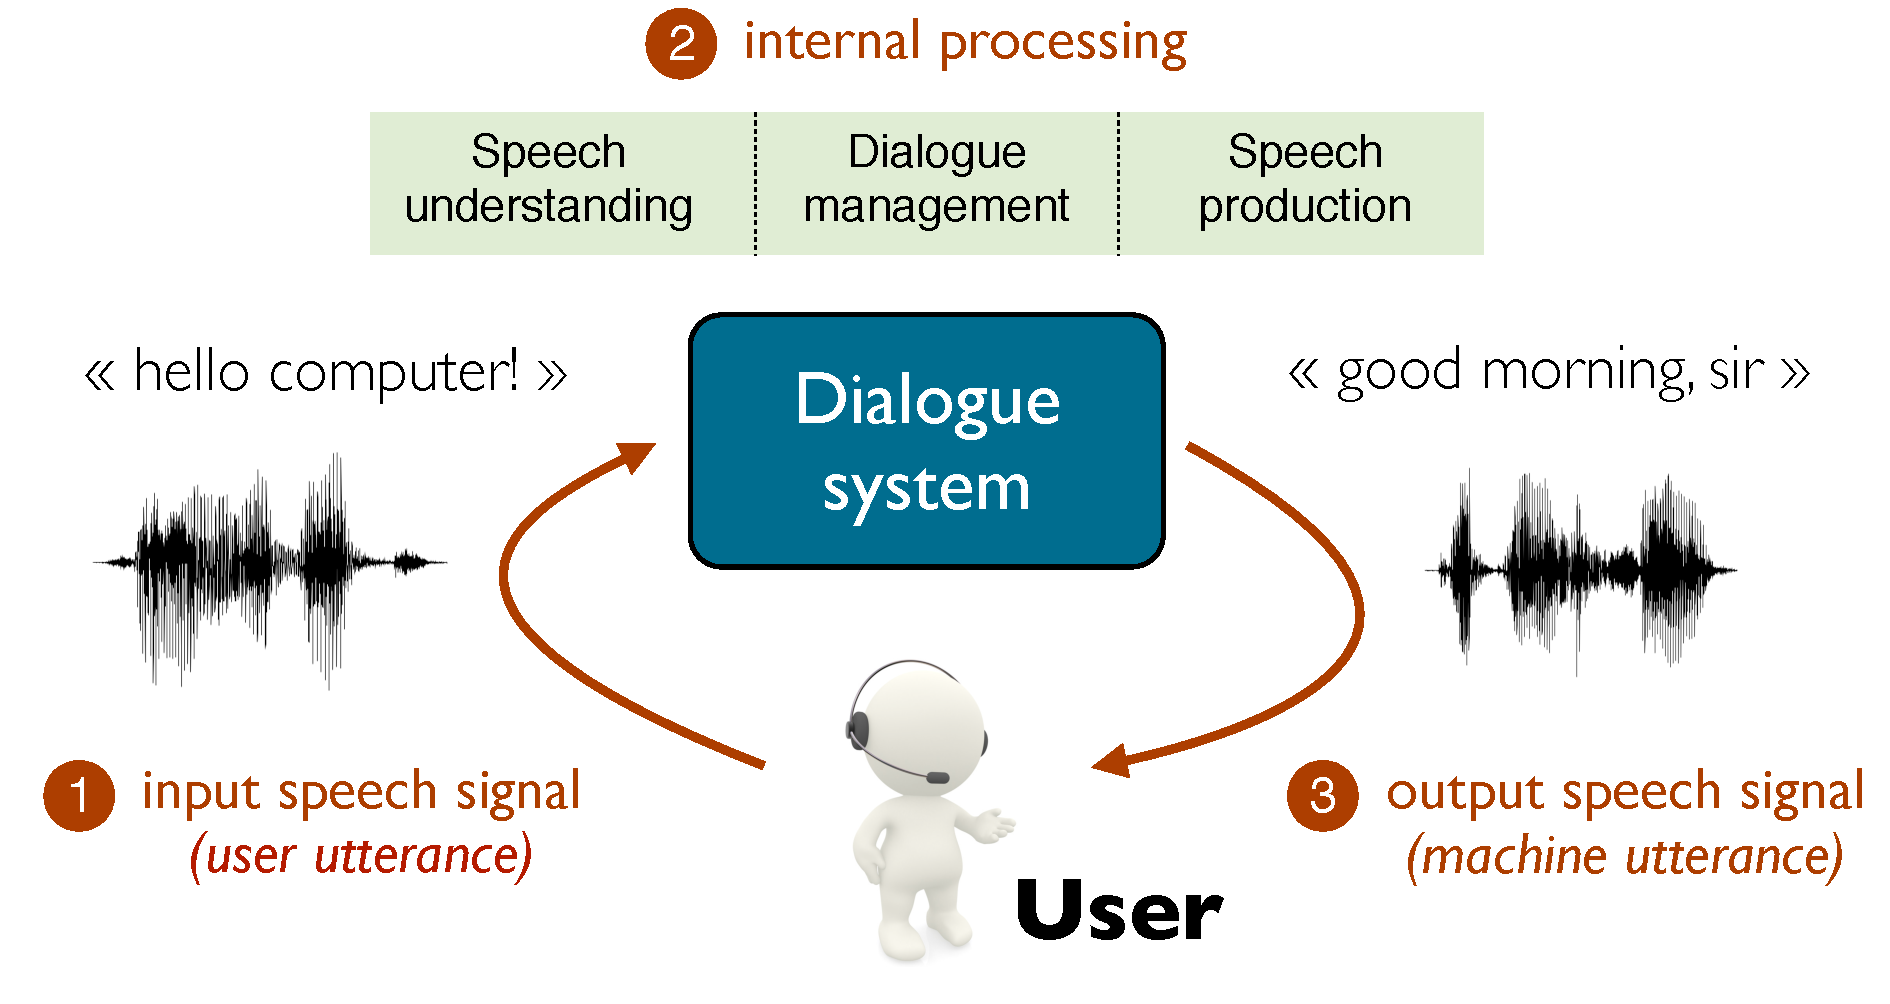
\includegraphics[scale=0.46]{imgs/basicsds.pdf}
\caption{Schematic view of a spoken dialogue system.}
\label{fig:basicsds}
\end{figure}

\section{Motivation}

Although spoken dialogue systems can greatly enhance the user interaction experience in many of today's technologies, their practical development can be a demanding enterprise. Speech is indeed much more complex than other types of (e.g.\ graphical or touch-based) user interfaces.

The present thesis concentrates on the problem of \textit{dialogue management}\index{dialogue management}.  Dialogue management is a central component in spoken dialogue systems and lies at the intersection between speech understanding and generation.  It serves a double role. Its first function is to maintain a representation of the current dialogue state\index{dialogue state}. This representation reflects the system knowledge of the current conversational situation, and often includes multiple features related to the dialogue history, the external context, and the tasks to perform.  This dialogue state is regularly updated with new information in the form of new user utterances or changes in the external context. 

The second function of dialogue management is to make decisions\index{action selection}.  Based on the current dialogue state, dialogue management must decide which actions to undertake. These actions are often communicative in nature (uttering a sentence), but can also pertain to non-verbal actions (e.g.\ waving or pointing in the case of human--robot interactions).  Dialogue management is therefore responsible for controlling the flow of the interaction, by (1) interpreting the user intentions in their context and (2) selecting which actions to perform given this context. In the example from Figure \ref{fig:basicsds}, this step corresponds to the decision of responding to the user utterance \utt{hello computer!} with another greeting action, \utt{good morning, sir}. 

Along with speech recognition, dialogue management is arguably one of the most difficult processing tasks in spoken dialogue systems. This difficulty stems from two defining characteristics of verbal interactions:
\begin{enumerate}
\item Verbal interactions are \textit{complex}.   Taking part in a dialogue requires tracking a multitude of factors, such as the interaction history, the hypothesised goals and preferences of the dialogue participants, and the external context. These factors depend on one another through multiple relations straddling the linguistic and extra-linguistic boundaries.  Selecting the action that is most appropriate in a particular situation is thus a difficult decision problem. 

\item Verbal interactions are also riddled with \textit{uncertainties}.  In order to make sense of a given dialogue, a conversational agent must handle numerous sources of uncertainty, including error-prone speech recognition, lexical,  syntactic and referential ambiguities, partially observable environments, and unpredictable interaction dynamics.  
\end{enumerate} 

The combination of these two properties forms an explosive mix.  In order to make sense of the interaction and act appropriately, the dialogue system must resort to sophisticated reasoning in order to interpret the user intentions in their context and plan the best course of action.  And it must do so under high levels of noise and uncertainty, where many pieces of information can be erroneous, missing, ambiguous, or fragmentary. This task is defined in the artificial intelligence literature as \textit{sequential decision-making under uncertainty}\index{sequential decision-making under uncertainty}, and is known to be a difficult computational problem, especially for domains as complex as spoken dialogue. Decision-making and action execution must also occur in real-time, since dialogue is by nature a real-time process. 

%\citep{Kaelbling:1998,aima2010}

Research on dialogue management can be divided into two main lines of investigation that reflect their focus on either of the two challenges we just mentioned.  

On the one hand, structural complexity is often dealt using conceptual tools borrowed from formal logic and classical planning\index{dialogue management!symbolic approaches to}.  These approaches provide principled methods for the interpretation and generation of dialogue moves through logical reasoning on the basis of a formal representation of the mental states of the dialogue participants (including their shared knowledge). Based on such representations, dialogue is then framed as a collaborative activity in which the dialogue participants work together to coordinate their actions, maintain a shared conversational context, resolve open issues and satisfy social obligations \citep{larsson2002,Jokinen:2009,Ginzburg2012}. These approaches can yield detailed analyses of various conversational behaviours, but they generally assume complete observability of the dialogue state and provide only a limited account of errors and uncertainties. In addition, they require the knowledge base on which the inference is grounded to be completely specified in advance by domain experts.  Their deployment in practical applications is therefore non-trivial. 

On the other hand, the problem of uncertainty is usually addressed by probabilistic modelling\index{probabilistic modelling} techniques \citep{Roy:2000,FramptonL09,Young:2010}.\index{dialogue management!statistical approaches to}  The state of the dialogue is here represented as a probability distribution over possible worlds.  This distribution represents the system's current knowledge of the interaction and is regularly updated as new observations are collected. These probabilistic models provide an explicit account for the various uncertainties that can arise during the interaction. They also enable the dialogue behaviour to be automatically optimised in a data-driven manner instead of relying on hand-crafted mechanisms.  Dialogue strategies can therefore be adapted to new environments or users without having to be reprogrammed. However, probabilistic models typically depend on large amounts of training data to estimate their parameters -- a requirement that is hard to satisfy for many dialogue domains.  Probabilistic models of dialogue are also usually limited to a handful of state variables and are difficult to scale to domains featuring rich conversational contexts. 

The work described in this thesis aims at reconciling these two strands of research through a new, hybrid framework to dialogue modelling and control. 

\section{Contributions}

The present thesis develops an original approach to dialogue management based on \textit{structured probabilistic modelling}.  The overarching motivation for this work is to design probabilistic models of dialogue that are scalable to rich interaction domains, yet only modest amounts of training data for their statistical optimisation.

An extensive body of work in the machine learning and decision-theoretic planning literature shows how to confront this issue by relying on more expressive representations, able to capture relevant aspects of the problem \textit{structure} in a compact manner. By taking advantage of hierarchical or relational abstractions, system designers can leverage their domain knowledge to yield probabilistic models which are both easier to learn (due to a reduced number of parameters) and more efficient to use (since the structure can be exploited by the inference algorithm).  

This thesis demonstrates how to translate these insights into dialogue modelling\index{dialogue modelling}.  The three central research questions of this thesis are:
\begin{enumerate}
\item How can we integrate prior domain knowledge into probabilistic models of dialogue?\index{dialogue management!domain knowledge in}
\item How can the parameters of these structured probabilistic models be estimated from data, using both supervised and reinforcement learning methods? \index{rule parameters!parameter estimation of} 
\item What is the empirical effect of such modelling techniques on the quality and efficiency of verbal interactions?
\end{enumerate}

\textit{Probabilistic graphical models} \citep{Koller+Friedman:09}\index{graphical models} constitute the theoretical foundations for a large part of our work.  Graphical models provide a generic, principled framework for representing and reasoning over complex probabilistic problems. They also come with well-defined data structures and general-purpose algorithms for model estimation and inference.  As shown in previous work \citep[see for instance][]{Thomson:2010:BUD:1772996.1773040}, one can elegantly represent the dialogue state as a Bayesian network\index{Bayesian network} (a well-known type of directed graphical model) factored in a set of state variables describing various aspects of the conversational situation.  The dialogue state is graphically depicted as a directed acyclic graph where the nodes correspond to particular variables and the edges are conditional dependencies between variables. To exploit such representation for decision-making tasks, the dialogue state can be extended with action and utility nodes that describe the utility for the agent of performing particular actions in a given situation. 

Statistically speaking, the estimation of such complex probabilistic structures is, however, a difficult endeavour, owing to the large number of variables and dependencies involved. The main novelty of our approach is the idea of representing the model distributions in a structured manner through the use of \textit{probabilistic rules}. \index{probabilistic rule} Probabilistic rules encode conditional distributions between variables in terms of structured mappings associating particular conditions expressed on a set of input variables to probabilistic effects on a set of output variables.  Utility distributions are also encoded in a similar manner. The conditions and effects of probabilistic rules are defined as first-order logical formulae. As new information becomes available to the dialogue manager, the Bayesian network representing the dialogue state is updated by instantiating the rules in the form of new nodes mediating between the input and output variables. Probabilistic rules are therefore employed as \textit{high-level templates} for the generation of a classical probabilistic model.  

The resulting modelling framework offers two major benefits. Most importantly, the reliance on more expressive representations can drastically reduce the number of parameters associated with the models.  Instead of being encoded through traditional probability tables, the conditional distributions between state variables are expressed through high-level rules that capture conditional dependencies with a compact set of parameters (one for each possible effect). As a consequence, these models are much easier to learn and generalise to unseen data.  In addition, the framework enables expert knowledge to be directly integrated in the probabilistic dialogue models. System developers can therefore exploit powerful abstractions to encode their prior knowledge of the dialogue domain in the form of pragmatic rules or task-specific assumptions.    
While the usefulness of domain-specific constraints has long been recognised, their use has most often been reduced to a mere external filter for classical statistical models \citep{heeman2007,williams2008}. By contrast, our approach incorporates such knowledge source in the very structure of the statistical model. 

We conducted several experiments to assess the validity of our approach in three distinct learning scenarios: \begin{enumerate} %, detailed in Section \ref{sec:wozlearning-experiments},

\item The first experiment focused on the problem of estimating action utilities given a small data set collected from Wizard-of-Oz interactions\index{Wizard-of-Oz interaction}.\footnote{A Wizard-of-Oz interaction is an experimental procedure borrowed from the field of human-computer interaction \citep{woz93}. In a Wizard-of-Oz study, the human subjects are asked to interact with a computer system that has all the appearances of reality, but is actually remotely controlled by an (unseen) human agent operating behind the curtains.  Wizard-of-Oz studies are often conducted to provide the system designers with interaction data from real users before the system is fully implemented.  The term is a cultural reference from the 1939 film ``The Wizard of Oz'' where an illusionist impersonates a powerful wizard by controlling an intimidating display from behind a curtain.}  Based on dialogue models encoded with probabilistic rules, the utilities of the different actions are learned through imitation learning. The experiment showed that the rule structure enabled the learning algorithm to converge faster and with better generalisation performance than unstructured models. This work was originally presented in \cite{rulebasedmodels-sigdial2012}. 
%, described in Section \ref{sec:rllearning-experiments},
\item The second experiment extended the above approach to reinforcement learning\index{reinforcement learning}. The goal of this study was to estimate the transition model of the domain from interactions with a user simulator. We compared the relative learning performance of two modelling approaches: one relying on unstructured distributions, and one based on probabilistic rules. The empirical results demonstrated the benefits of capturing the domain structure with probabilistic rules. The results were first published in \cite{interspeech2013}. 
\item Finally, the third and final experiment was designed to evaluate the empirical effect of the modelling framework through a user evaluation in a human--robot interaction domain. The experiment compared three alternative dialogue management methods: a purely hand-crafted approach (based on a finite-state automaton), a purely statistical approach (based on factored models) and a hybrid approach based on probabilistic rules. The rule-structured approach was shown to outperform the two baseline methods on a range of quality metrics, including both objective metrics extracted from the interaction logs and subjective metrics derived from responses to a user survey. \index{user evaluation}
\end{enumerate}

An additional contribution of this thesis is the development of a software toolkit that implements all the data structures and algorithms presented in this work. The toolkit is called \opendial{}\index{openDial@\opendial{}}  and is freely available under an open source licence.\footnote{The toolkit can be downloaded at \urlsmall{http://opendial.googlecode.com}.} The purpose of the toolkit is to enable system developers to design and evaluate dialogue systems based on probabilistic rules. All domain-specific knowledge is declaratively specified in the rules for the domain. The system architecture is therefore reduced to a small set of core algorithms for accessing and updating the dialogue state \citep{lison-semdial2012}. This architectural design makes the toolkit fully generic and domain-independent. The \opendial{} toolkit comes with a user interface allowing developers to interactively test their system and visualise how the internal dialogue state is evolving over time.  % Its implementation is described in Chapter \ref{chap:opendial}. 

We carried out all the experiments described in this thesis in a particular application domain, namely \textit{human--robot interaction} \index{human--robot interaction} (HRI).  The choice of this application domain as a test bed for our framework was motivated by two factors.  The first factor is the presence of a complex situated environment in which the agent must complete its tasks.  This dialogue context\index{dialogue context} is highly dynamic -- for instance, the physical position of objects and persons may change in the course of the interaction, and the system tasks are regularly altered as a result of the coordinated actions of the robot and human user. The second factor relates to the occurrence of multiple sources of uncertainty caused by imperfect sensory devices, unreliable motors, and failure-prone speech recognition. This combination of a rich conversational context and high levels of uncertainty is precisely the focus of the present work and justifies the selection of  human--robot interaction as a test bed to evaluate the performance of our modelling approach in real settings.

\begin{wrapfigure}[13]{r}{60mm}
\vspace{-6mm}
\centering 
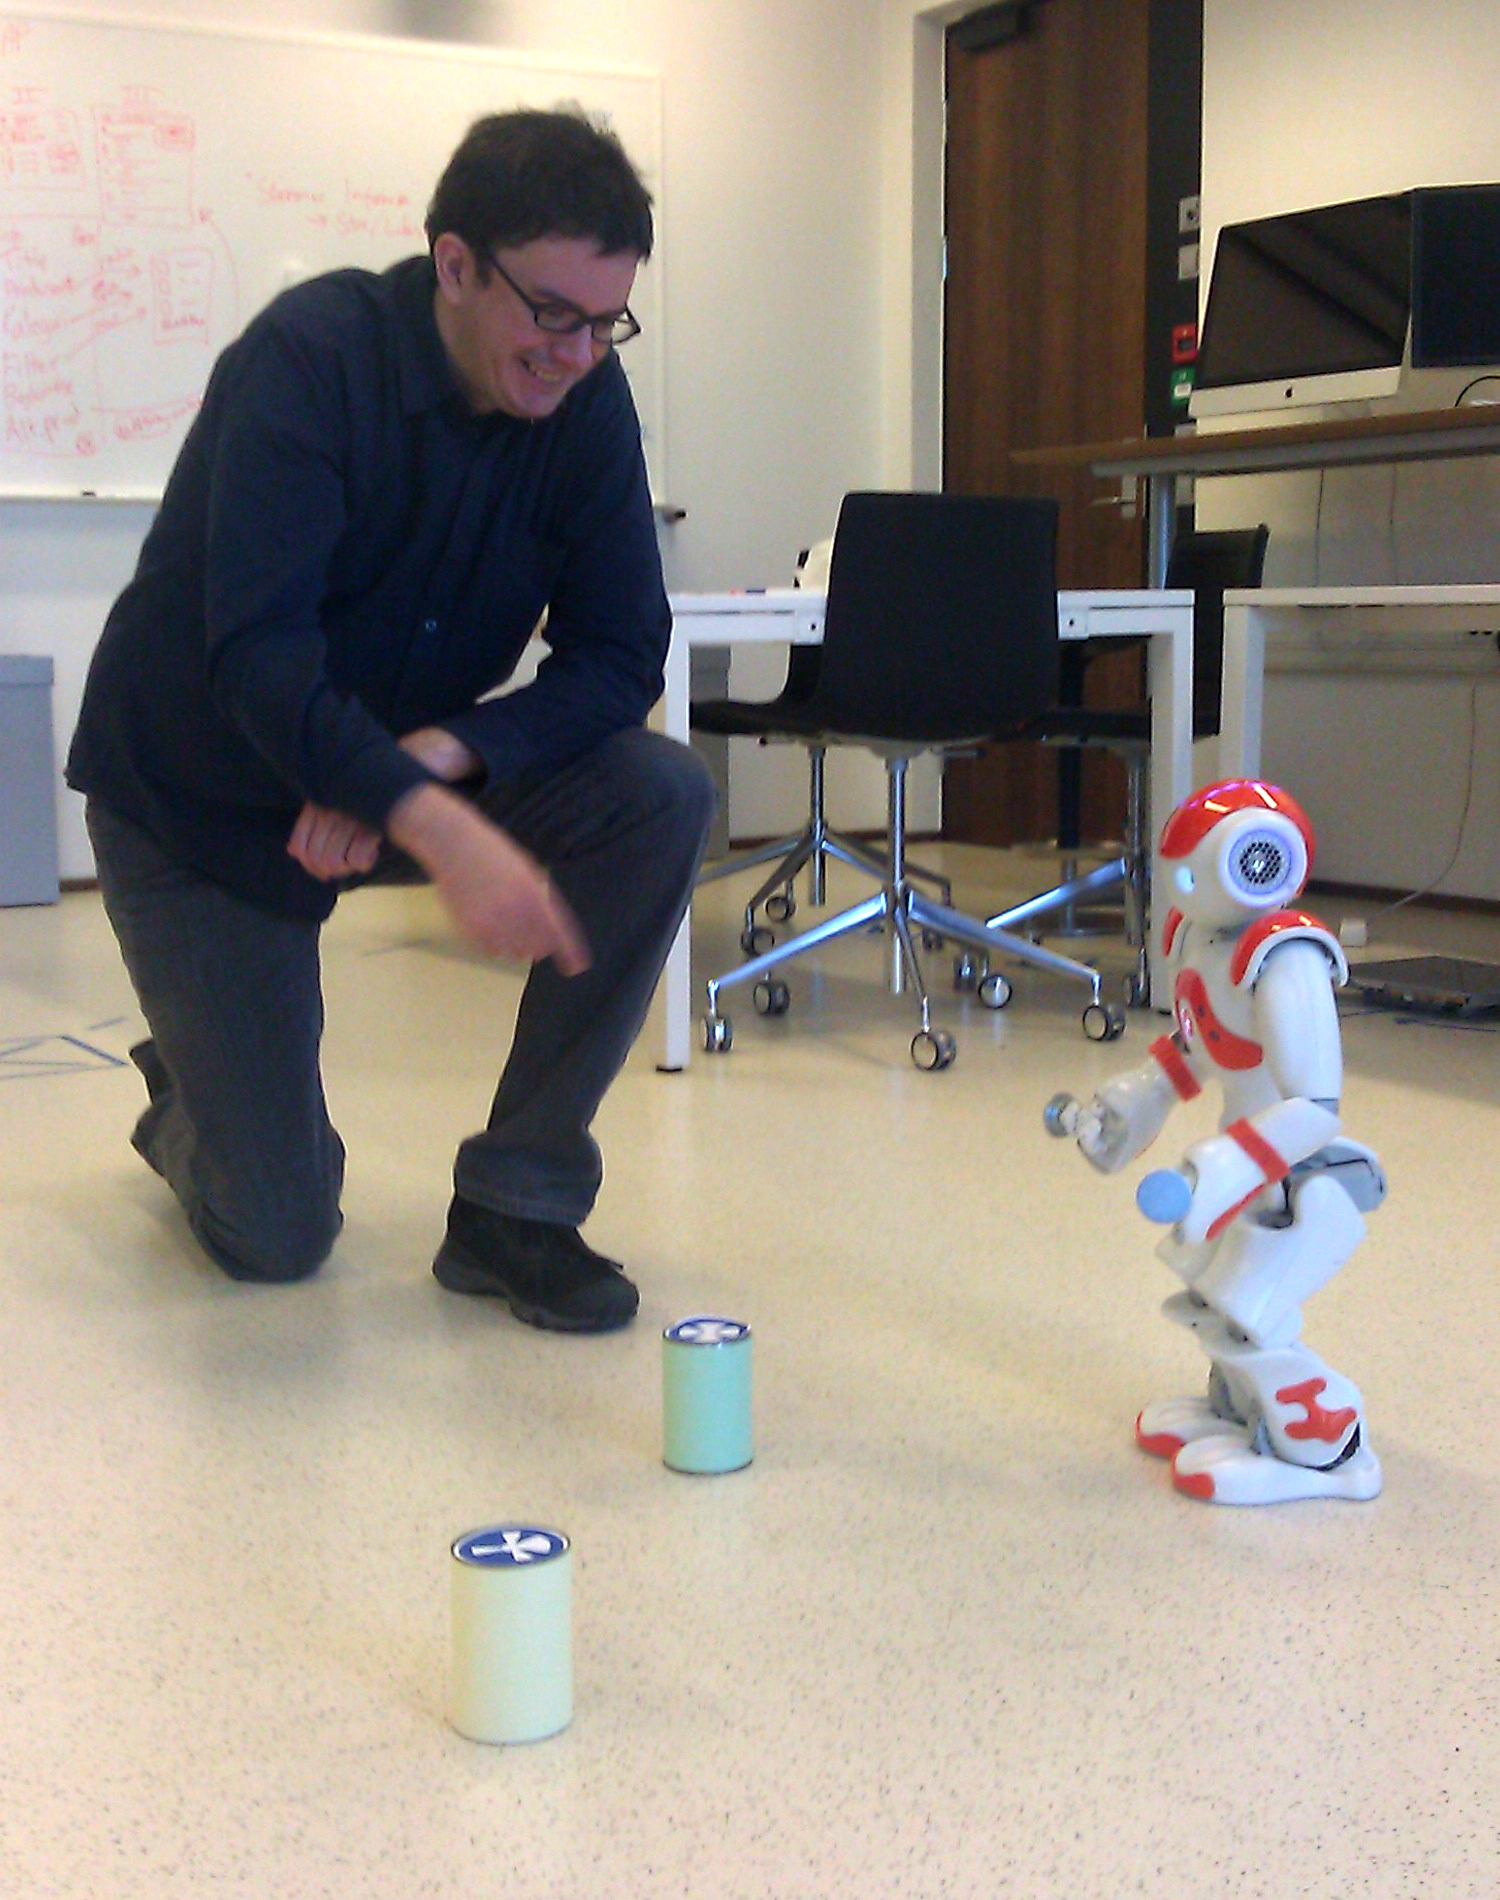
\includegraphics[scale=0.1]{imgs/nao1.jpg}
\caption{Human user interacting with the Nao robot.}
\label{fig:nao}
\end{wrapfigure}

The Nao robot V4 (NextGen) \index{Nao robot} manufactured by Aldebaran Robotics\footnote{cf.  \urlsmall{http://www.aldebaran-robotics.com}.} was used as a development and testing platform in all our experiments. An example of interaction with the robot is shown in Figure \ref{fig:nao}.  Most of our experiments involved the Nao robot conversing with a human user in a shared visual environment featuring a few basic objects that can be both perceived and grasped by the robot.  The interactions typically revolved around the completion of a few simple tasks such as moving objects from one position to another under the supervision of the human user. Chapters \ref{chap:wozlearning}--\ref{chap:user-evaluation} provide a detailed description of the interaction scenarios, data collection and evaluation setups followed for the experiments.

% combination of theory + experiments and implementation? 

\section{Outline of the thesis}

A brief overview of the thesis structure, chapter by chapter, is provided below. 

\begin{description}
  \item[\textbf{Chapter \ref{chap:background}: Background}] \hfill  \vspace{2mm}
  
This chapter introduces the fundamental concepts and methods used throughout this thesis. We start with an overview of some of the core linguistic properties of dialogue and describe key notions such as turn-taking, dialogue acts and grounding.  We then describe a range of software architectures employed to design spoken dialogue systems and the role of each component within them.  We also mention a range of important applications for spoken dialogue systems. Finally, we survey the various approaches that have been put forward in the research literature to address the dialogue management problem, including both hand-crafted and statistical methods. \vspace{2mm}

  \item[\textbf{Chapter \ref{chap:probmodelling}: Probabilistic modelling of dialogue}] \hfill \vspace{2mm}

 The chapter starts by reviewing the core notions of directed graphical models, which constitute the formal basis for our framework.  We define how Bayesian networks are constructed, and show how they can be augmented to capture temporal sequences and decision-theoretic problems. We also briefly describe the most important algorithms for learning and inference based on such models.  We then  move to the field of reinforcement learning and spell out its most central elements, such as Markov Decision Processes, value functions and policies. We also examine how reinforcement learning methods can be extended to partially observable settings, since dialogue is a prototypical example of decision-making under partial observability.  Finally, the last section translates these concepts and methods to the field of dialogue management, and discusses both supervised and reinforcement learning approaches to the optimisation of dialogue policies.
 
  \item[\textbf{Chapter \ref{chap:rules}: Probabilistic rules}] \hfill \vspace{2mm}
 
  This chapter lays down the central concepts and algorithms of our own modelling approach to dialogue management. We define what probabilistic rules are and how they are internally structured through conditions and effects.  We describe two main types of rules, used to respectively encode probability and utility distributions. We then explain how the rules are practically instantiated in the Bayesian network representing the dialogue state, as well as the algorithms employed to update the dialogue state and perform action selection. The chapter also addresses some advanced modelling questions related to the manipulation of special data structures such as lists and strings, and concludes by comparing our framework to previous work. \vspace{2mm}
  
  \item[\textbf{Chapter \ref{chap:wozlearning}: Learning from Wizard-of-Oz data}] \hfill  \vspace{2mm}
  
 This chapter shows how the parameters attached to probabilistic rules can be automatically learned from training data, in a supervised learning fashion. The algorithm used for estimating the rule parameters is grounded in Bayesian learning techniques.  To validate our approach, we detail an experiment on a statistical estimation task based on Wizard-of-Oz data collected in a human--robot interaction domain.  The experiment illustrates the benefits of probabilistic rules compared to unstructured distributions.  \vspace{2mm}

\item [\textbf{Chapter \ref{chap:rllearning}: Learning from interactions}] \hfill  \vspace{2mm}

Chapter \ref{chap:rllearning} extends parameter estimation to a reinforcement learning context.  We show how the parameters of rule-structured dialogue models can be efficiently learned from observations collected during the interaction itself, without having access to any gold standard annotations.  The procedure follows a Bayesian reinforcement learning approach and can be applied to optimise the rule parameters using both model-based and model-free variants. Finally, we report the results of two experiments carried out with a user simulator.  The experiments concentrated on the estimation of the transition model for a human--robot interaction domain, and evaluated the relative performance of a rule-structured model compared to a plain statistical model as well as the learning efficiency of model-based vs. model-free methods.   \vspace{2mm}


\item [\textbf{Chapter \ref{chap:opendial}: Implementation}] \hfill  \vspace{2mm}

Chapter \ref{chap:opendial} uncovers how the various algorithms and data structures presented in this thesis are technically integrated in the system architecture.  We explain how the \opendial{} toolkit is structured, describe how dialogue domains are practically specified in a generic XML format and discuss the implementation and performance tuning of the algorithms used for probabilistic inference and online planning.  We also compare the \opendial{} architecture to related software frameworks.  Finally, the chapter presents the integrated dialogue system employed to carry out the experiments in this thesis and the graphical user interface developed to visualise the evolution of the dialogue state over the course of the interaction. 

\item [\textbf{Chapter \ref{chap:user-evaluation}: User evaluation}] \hfill  \vspace{2mm}

This chapter presents an extensive user evaluation of our approach in a human--robot interaction domain with 37 participants.  The evaluation contrasted the empirical performance of three dialogue management strategies: a hand-crafted approach expressed as a finite-state automaton, a statistical approach based on factored models, and a hybrid approach encoded with probabilistic rules (the two latter models being estimated on the basis of a small set of Wizard-of-Oz interactions).  The empirical results show that the use of rule-structured models yields significant improvements in both objective and subjective metrics of interaction quality compared to the two baselines. \vspace{2mm}


\item [\textbf{Chapter \ref{chap:conclusions}: Concluding remarks}] \hfill  \vspace{2mm}

The final chapter concludes this dissertation with a summary of the presented research contributions, followed by an outline of future work.   \vspace{2mm}

\end{description}

